\chapter{Analýza požadavků pro práci s~knihovnou GTTG}
\label{kap:spec}
Z~kapitoly \ref{kap:uvod} jsme získali základní představu o~tom, jaký účel bude knihovna GTTG splňovat a~určili jsme si cíle, kterými se při implementaci knihovny budeme řídit. V~této kapitole si tyto cíle více upřesníme a~vytvoříme detailní souhrn požadavků, představujících kritéria pro správný výběr implementace. Požadavky je možné rozdělit do dvou hlavních kategorií:

\begin{itemize}
	\item Požadavky na chování grafické komponenty jako okna, v~kterém je zobrazován nákresný jízdní řád 
	\item Požadavky na vykreslování nákresného jízdního řádu a~práci s~jeho obsahem
\end{itemize}

\section{Požadavky na chování grafické komponenty}
\label{kap:spec:komponenta}
V~této části vytvoříme požadavky určující chování grafické komponenty, která představuje okno s vykreslovaným obsahem. Určíme, jak se komponenta chová, například v~rámci integrace s~uživatelským rozhraním. Určením požadavků pro práci s~touto komponentou vytvoříme prostředí, které umožní práci s~nákresným jízdním řádem. Při určování těchto požadavků jsme zejména brali ohled na náš cíl zajistit replikovatelnost chování původních aplikací. Narozdíl od původních aplikací by ale knihovna měla nabízet i~nové chování, které by zlepšilo interakci uživatelů s~komponentou.

\subsubsection*{Interakce uživatelů s~komponentou}
Jelikož vytváříme knihovnu pro více aplikací, měli bychom podporovat co největší množinu operací, kterými lze komponentu modifikovat. Aplikace pracující s~knihovnou si z~této množiny operací vybere pouze ty, které chce podporovat. V~této části určíme požadavky, které umožní interakcemi uživatele s~komponentou měnit zobrazovaný obsah komponenty. Podívejme se, jak existující aplikace zmíněné v~podkapitole \ref{aplikace_gvd} umožňují uživatelům pracovat s~komponentou. Na obrázku \ref{fig:spec:oltis_grafikon} se nachází aplikace od OLTIS Group. Na pravé hraně komponenty nabízí posuvník pro změnu zobrazované části traťového úseku. Stejným způsobem komponenta umožňuje na horizontále výběr zobrazovaného časového intervalu. Uživateli je tak zobrazen jen nějaký výřez z~celého obsahu nákresného jízdního řádu, který vytváří hranice, v~rámci kterých je možné zobrazení měnit posuvníky. Grafické znázornění hranic a~zobrazované části nákresného jízdního řádu v~komponentě se nachází na obrázku \ref{fig:spec:border}. Jelikož se stejným způsobem chovají i~ostatní existující aplikace a~toto chování chceme zachovat i~u~nových aplikací pracujících s~knihovnou, definujeme následující požadavky.

\begin{enumerate}[label=\color{reqcolor}\textbf{R{\arabic*}}]
	\item \label{spec:req:interaction_trans1} Komponentou zobrazovaný obsah se nachází v~ohraničení, které je určeno zobrazitelným obsahem nákresného jízdního řádu
	\item \label{spec:req:interaction_trans2} Komponentou zobrazovaný obsah je možné měnit posunem po vertikální a~horizontální ose v~rámci ohraničení definovaném \ref{spec:req:interaction_trans1}
\end{enumerate}

\begin{figure}[!htb]
	\centering
	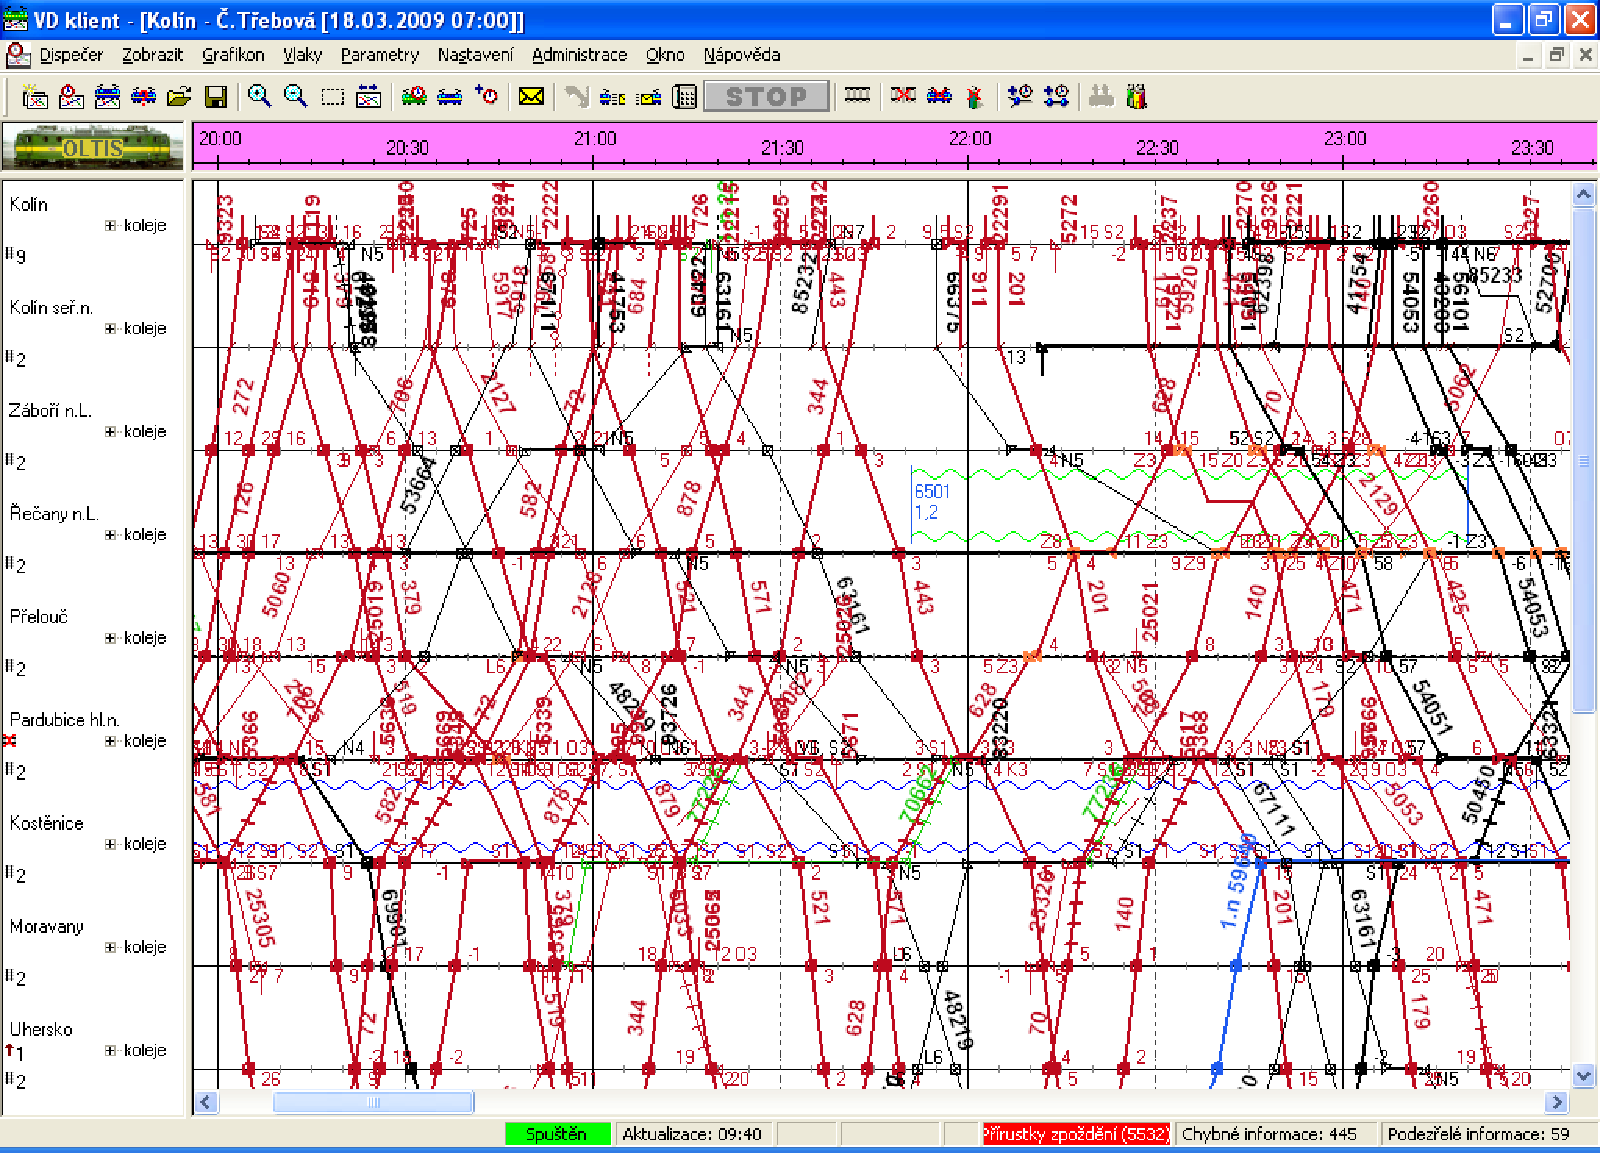
\includegraphics[width=0.9\textwidth]{../img/kap1_ISOR_window}
	\caption{Aplikace od OLTIS Group s~posuvníky, převzato ze stránky společnosti~\cite{ISOR_CDS}}
	\label{fig:spec:oltis_grafikon}
\end{figure}

\begin{figure}[!htb]
	\centering
	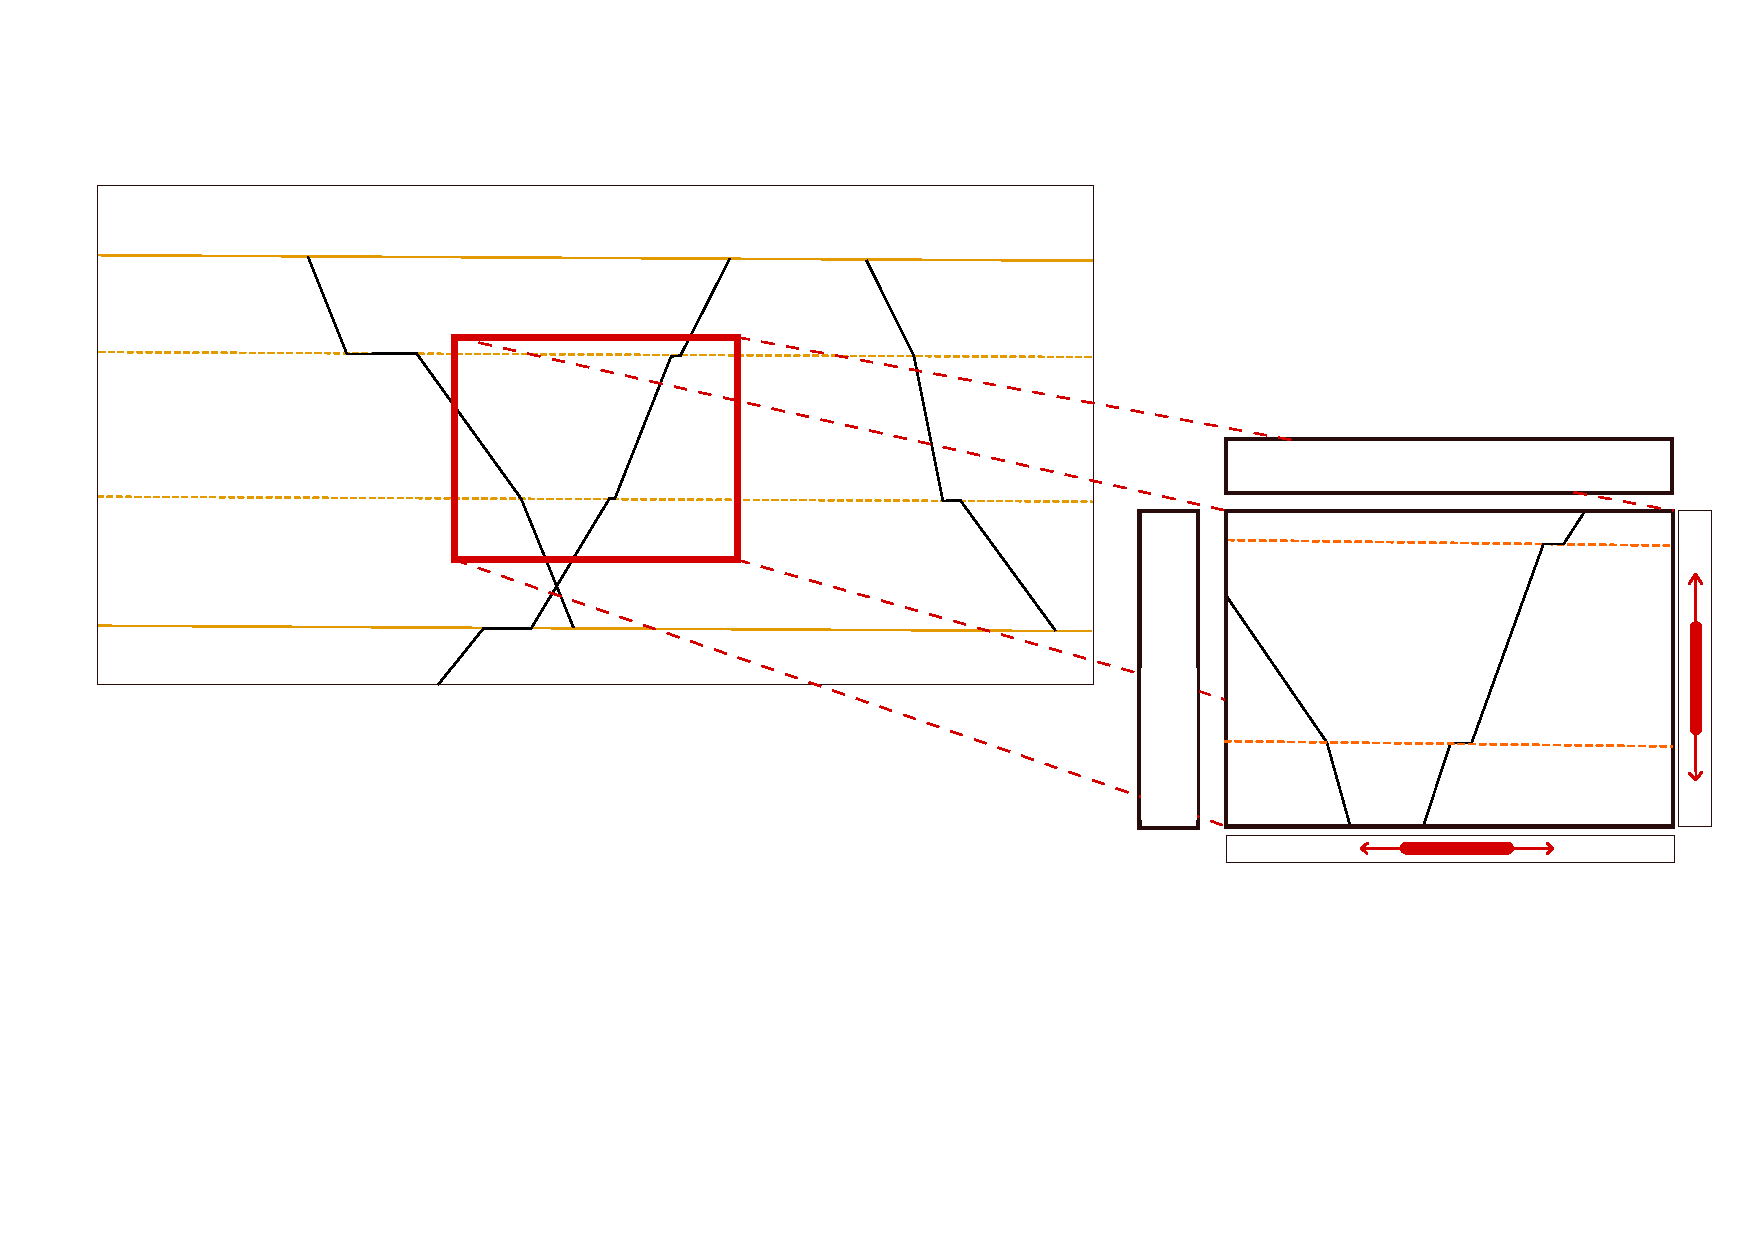
\includegraphics[width=0.9\textwidth]{../img/kap2_ohraniceni_definice}
	\caption{Komponentou zobrazovaný obsah a~ohraničení určené zobrazitelným obsahem nákresného jízdního řádu}
	\label{fig:spec:border}
\end{figure}

\pagebreak
Existující aplikace umožňují měnit zobrazený obsah pouze posunem. Interakci uživatelů s~grafickou komponentou bychom chtěli zlepšit přidáním možnosti zobrazovaný obsah přiblížit a~oddálit, jak je ukázáno na obrázku \ref{fig:spec:zoom}. Pohled se bude oddalovat nebo přibližovat vůči zobrazovanému bodu, jehož umístění na plátně bude stále stejné -- v~případě, že uživatel bude zobrazení přibližovat myší, bude tento bod odpovídat kurzoru myši. V~případě, že operace oddálení způsobí, že by se komponenta nacházela mimo ohraničení zabrazitelného obsahu a~porušila by požadavek \ref{spec:req:interaction_trans1}, je potřeba vzniklou situaci deterministicky opravit. Případ, kdy k~takové situaci dochází, je uveden na obrázku \ref{fig:spec:zoom_out_of_bounds}.
\pagebreak
\begin{enumerate}[label=\color{reqcolor}\textbf{R{\arabic*}},resume]
	\item \label{spec:req:interaction_zoom1} Komponenta podporuje operace přiblížení a~oddálení pohledu. Při těchto operacích je určen v~zobrazení bod, který po operaci v~komponentě nezmění svou polohu
	\item \label{spec:req:interaction_zoom2} V~případě, že by se oddálení komponenty dostalo mimo ohraničení definované v~\ref{spec:req:interaction_trans1}, použije knihovna deterministický postup, který operaci oddálení vhodně opraví
\end{enumerate}

\begin{figure}[!htb]
	\centering
	\includegraphics[width=0.9\textwidth]{../img/kap2_scale_example}
	\caption{Přiblížení pohledu na bod v~komponentě, kde se nachází kurzor myši. Tento bod zůstává po přiblížení v~komponentě na stejném místě.}
	\label{fig:spec:zoom}
\end{figure}

\begin{figure}[!htb]
	\centering
	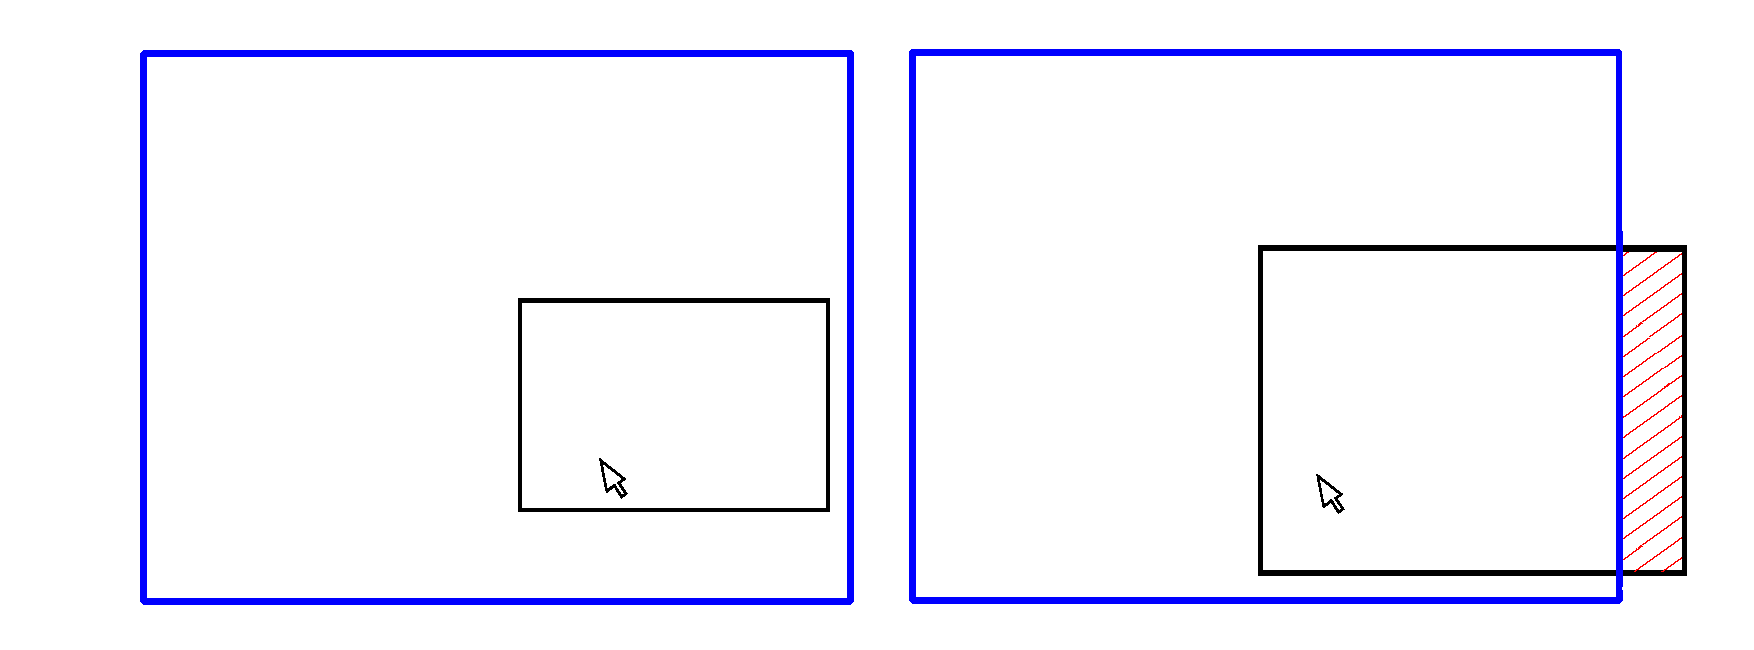
\includegraphics[width=0.9\textwidth]{../img/kap2_scale_example_out_of_bounds}
	\caption{Situace, kdy se komponenta po oddálení nachází mimo ohraničení definované \ref{spec:req:interaction_trans1}.}
	\label{fig:spec:zoom_out_of_bounds}
\end{figure}

\subsubsection*{Mapování časových intervalů na horizontální osu}
\label{kap2:time_intervals}
Víme, že horizontální osa grafu, v~němž je nákresný jízdní řád umístěn, značí čas. V~nákresném jízdním řádu pak zobrazujeme provoz z~nějakého časového intervalu určeného právě časy na horizontální ose. Pokud zobrazujeme výřez z~nákresného jízdního řádu, časový interval tohoto výřezu je podinterval zmíněného časového intervalu. Znázornění těchto intervalů se nachází na obrázku \ref{fig:spec:casove_intervaly}. Jelikož se zmíněnými intervaly budeme často pracovat, zavedeme jejich označení:

\begin{enumerate}[label=\color{reqcolor}\textbf{R{\arabic*}},resume]
	\item \label{spec:req:int1} Komponenta mapuje časový interval, který se nazývá \textit{časový interval zobrazení}, na body horizontální osy komponenty
	\item \label{spec:req:int2}	Komponenta mapuje časový interval, který se nazývá \textit{časový interval ohraničení}, na body horizontální osy v~rámci ohraničení definovaného \ref{spec:req:interaction_trans1}
\end{enumerate}

\begin{figure}[!htb]
	\centering
	\includegraphics[width=\textwidth]{../img/kap2_time_intervals}
	\caption{Časový interval zobrazení (červeně) a~ohraničení (modře).}
	\label{fig:spec:casove_intervaly}
\end{figure}

\subsubsection*{Změna velikosti komponenty a~hranic obsahu}
Jelikož bude komponenta obvykle součástí uživatelského rozhraní, může být její velikost v~rámci procesu rozmístění uživatelského rozhraní změněna. Na obrázku \ref{fig:spec:zmena_velikosti_horizontalni} je zobrazena změna šířky komponenty. Pokud porovnáme původní a~nové zobrazení po změně, vidíme, že se časový interval zobrazení nezměnil. Existující aplikace se při změně šířky komponenty chovají stejným způsobem, bude to tedy chování komponenty, které od knihovny při změně šířky požadujeme.

\begin{enumerate}[label=\color{reqcolor}\textbf{R{\arabic*}},resume]
	\item \label{spec:req:width_mod1} Při změně velikosti komponenty zůstává časový interval zobrazení definovaný \ref{spec:req:int1} nezměněn
\end{enumerate}

\begin{figure}[!htb]
	\centering
	\includegraphics[width=\textwidth]{../img/kap2_horizontal_resize}
	\caption{Nezměněný časový interval při změně šířky komponenty}
	\label{fig:spec:zmena_velikosti_horizontalni}
\end{figure}

Při změně výšky komponenty existuje více způsobů, jak zobrazení upravit. Jednou z~možností je použít stejné chování, které se používá při změně šířky komponenty. Zobrazovaný obsah by tak zůstal stejný -- v~nejjednodušším scénaři budou dopravní body v~komponentě rozmístěny podle poměru jejich kilometrické vzdálenosti. Chování je znázorněno na obrázku \ref{fig:spec:zmena_velikosti_vertikalni_modifikace_1}.

\begin{enumerate}[label=\color{reqcolor}\textbf{R{\arabic*}},resume]
	\item \label{spec:req:height_mod1}	Při změně výšky komponenty může zůstat zobrazovaný obsah komponenty nezměněn a~jeho rozmístění je vzhledem k~nové výšce proporčně upraveno
\end{enumerate}

\begin{figure}[!htb]
	\centering
	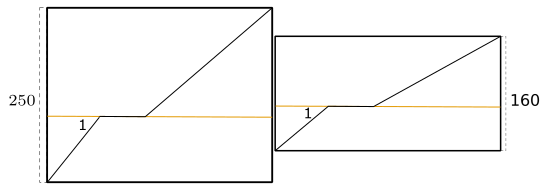
\includegraphics[width=\textwidth]{../img/kap2_vertical_resize_proportional}
	\caption{Proporční rozmístění stejného obsahu při změně výšky komponenty}
	\label{fig:spec:zmena_velikosti_vertikalni_modifikace_1}
\end{figure}

Problémem předchozího požadavku je chování v~případě, kdy je výška komponenty příliš malá. Zobrazované informace v~komponentě jsou pak nepřehledné. Proto chceme vedle tohoto řešení nabídnout jiné, které zachová původní rozmístění. V~případě zmenšení výšky se ze zobrazovaného obsahu zobrazí jeho výřez a~nově skrytou část původního obsahu je možné zobrazit posunutím. Při zvětšení výšky se k~původnímu obsahu přidá doposud skrytá zobrazitelná část navazující na původní obsah. Zvětšení výšky je možné tímto způsobem aplikovat, pokud je komponenta stále umístěna v~hranicích zobrazitelného obsahu. Chování je znázorněno na obrázku \ref{fig:spec:zmena_velikosti_vertikalni_modifikace_2}.

\begin{enumerate}[label=\color{reqcolor}\textbf{R{\arabic*}},resume]
	\item \label{spec:req:height_mod2} Je možné zmenšit výšku komponenty tak, aby byla zobrazena jen část původního výřezu
	\item \label{spec:req:height_mod3} Je možné zvětšit výšku komponenty tak, aby byla zobrazena původní část s~nově odkrytou částí obsahu. Modifikace je možná, pokud zvětšení komponenty nepřekročí ohraničení definované \ref{spec:req:interaction_trans1}
\end{enumerate}

\begin{figure}[!htb]
	\centering					
	\includegraphics[width=\textwidth]{../img/kap2_vertical_resize_view_change}
	\caption{Změna zobrazeného obsahu při změně výšky komponenty}
	\label{fig:spec:zmena_velikosti_vertikalni_modifikace_2}
\end{figure}

\subsubsection*{Modifikace časových intervalů}
\label{kap2:modifikace_cas_intervaly}
V~této části popíšeme už zavedené modifikace ve formě nastavování časových intervalů. Je užitečné, aby zobrazovaný obsah, odpovídající nějakému časovému intervalu, bylo možné podle určení tohoto intervalu nastavit. Uvedeme si příklad, kdy se tento způsob modifikace uplatňuje. Aplikace často nabízí možnost zobrazit obsah v~přednastavených úsecích několika hodin (například 2h, 4h, 6h). Pokud například komponenta zobrazuje interval o~délce dvě hodiny (14:00 - 16:00), je možné změnit obsah komponenty tak, aby nyní zobrazoval interval šesti hodin (12:00 - 18:00). Tato modifikace je zachycena na obrázku \ref{fig:spec:zmena_casoveho_intervalu_zobrazeni}. Pokud toto chování zobecníme, požadujeme, aby mohl být nastaven jakýkoliv podinterval časového intervalu ohraničení.

\begin{enumerate}[label=\color{reqcolor}\textbf{R{\arabic*}},resume]
	\item \label{spec:req:time_mod1} Zobrazení může být změněno tak, aby obsah komponenty odpovídal zobrazení nově nastavovaného časového intervalu zobrazení, který musí být součástí časového intervalu ohraničení
\end{enumerate}

\begin{figure}[!htb]
	\centering					
	\includegraphics[width=\textwidth]{../img/kap2_time_interval_change}
	\caption{Změna časového intervalu zobrazení}
	\label{fig:spec:zmena_casoveho_intervalu_zobrazeni}
\end{figure}

Existují případy, kdy se v komponentě zobrazuje obsah odpovídající aktuálnímu času v~rámci nějakého časového intervalu (například okno 12:00 - 18:00 s~aktuálním časem 15:00). Periodicky se pak například po hodině celé toto časové okno o~hodinu posune. Chtěli bychom proto umožnit i~změnu časového intervalu ohraničení.

\begin{enumerate}[label=\color{reqcolor}\textbf{R{\arabic*}},resume]
	\item \label{spec:req:time_mod2} Zobrazitelný obsah je možné změnit nastavením nového časového intervalu ohraničení. V~rámci změny časového intervalu ohraničení je nutné poskytnout podinterval, který bude nastaven jako časový interval zobrazení
\end{enumerate}

Navíc se knihovna musí jednotně chovat ve změně vertikální polohy komponenty v~rámci ohraničení při změně časového intervalu. Jako nejvhodnější se ukazuje vertikální umístění komponenty neměnit, jelikož můžeme změnou časového intervalu vytvořit posun, zobrazující část původních informací z~výřezu na stejné vertikální úrovni.

\begin{enumerate}[label=\color{reqcolor}\textbf{R{\arabic*}},resume]
	\item \label{spec:req:time_mod3} Změny zobrazení určené časovými intervaly nemění vertikální umístění komponenty v~ohraničení definovaném \ref{spec:req:interaction_trans1}
\end{enumerate}

\subsubsection*{Podporované jednotky určující velikost komponenty}
Doposud jsme neurčili, v~jakých jednotkách se měří velikosti komponenty a~jejího ohraničení. Jelikož komponenta zobrazuje nějaké plátno, které je určeno jednotkami pixelů, požadujeme, aby s~jejími velikostmi bylo možné pracovat v~různých jednotkách pixelů -- například jednotkách pixelů nezávislých na zařízení a~jednotkách pixelů zařízení. Pokud by se vývojář rozhodl používat jednotky pixelů zařízení, knihovna by mu měla poskytnout možnost zjistit aktuální DPI\footnote{dots per inch} hodnotu zařízení, na kterém je aplikace spuštěna, aby mohl případně zajistit třeba stejnou velikost textu mezi různými zařízeními.

\begin{enumerate}[label=\color{reqcolor}\textbf{R{\arabic*}},resume]
	\item \label{spec:req:unit1} Velikost komponenty může být udávána v~různých jednotkách pixelů:
		\begin{itemize}
			\item	Jednotky pixelů nezávislých na zařízení
			\item	Jednotky pixelů zařízení
		\end{itemize} 
	\item \label{spec:req:unit2} V~případě práce s~jednotkami pixelů zařízení bude mít vývojář možnost zjistit hodnotu DPI zařízení  
\end{enumerate}

\subsubsection*{Stav pro určení zobrazovaného obsahu}
Předchozími požadavky jsme vytvořili základ pro prostředí, v~kterém je možné pracovat se zobrazením nákresného jízdního řádu. Toto prostředí je popsáno informacemi, které tvoří jeho stav.

\begin{enumerate}[label=\color{reqcolor}\textbf{R{\arabic*}},resume]
\item \label{spec:req:state} Aby bylo možné určit, jaký obsah se má v~komponentě zobrazit, zahrne komponenta do svého stavu:
	\begin{itemize}
		\item Velikosti komponenty a~ohraničení
		\item Umístění komponenty v~ohraničení definovaném \ref{spec:req:interaction_trans1}
		\item Faktor škálování, který určuje, jak moc je zobrazení v~komponentě přiblížené a~odpovídá násobkům neupravené velikosti
		\item Časový interval zobrazení a~časový interval ohraničení
	\end{itemize}
\end{enumerate}

\section{Vykreslení obsahu nákresných jízdních řádů}
\label{kap:spec:obsah_njr}
Tato část určuje požadavky, které souvisí s~vykreslováním obsahu komponenty, jejíž chování jsme určili požadavky předchozí části. Dále uvedeme požadavky, které vývojáři ulehčí přípravu nákresného jízdního řádu k~jeho vykreslení. Tyto požadavky nejsou tak přesné jako v~předchozí části, ale spíše určují směr, jakým se implementace knihovny musí vydat, aby mohla být dostatečně rozšiřitelná a~využitelná implementacemi více typů nákresných jízdních řádů.

\subsection*{Plátno pro kreslení}
Knihovna by měla vývojářům ulehčit práci při vykreslování nákresného jízdního řádu. Změnou stavu komponenty se neustále mění obsah, který by měl být zobrazen. Při každé změně je potřeba na komponentě zobrazit nově odpovídající část z~celého nákresného jízdního řádu. Pokud bychom po knihovně požadovali co nejméně, stačilo by, aby vývojáři byla dostupná informace o~stavu komponenty určena v~\ref{spec:req:state} a~plátno, jehož obsah je zobrazen v~komponentě. Vývojář by pak musel spočítat, jaký obsah se má zobrazit a~tento obsah vykreslit. Takový přístup je ale pro vývojáře knihovny velmi náročný. Knihovna by mu měla nabídnout plátno, na které by se zobrazil celý obsah nákresného jízdního řádu a~knihovna by pak sama přepočítala, jaký výřez z~plátna se má v~komponentě zobrazit.

Knihovna by ale měla nabízet i~možnost pracovat pouze s~částí plátna, která je zobrazena v~komponentě. Tato změna je užitečná v~případě, pokud chceme v~komponentě zobrazit informace, které nejsou součástí nákresného jízdního řádu, ale mají informativní charakter v~rámci aplikace, jako je současné datum nebo notifikace o~změně související s~nákresným jízdním řádem. Během kreslení tak může uživatel pohled na plátno měnit.

\begin{enumerate}[label=\color{reqcolor}\textbf{R{\arabic*}},resume]
	\item \label{spec:req:canvas1} Uživateli je přístupné plátno, které odpovídá obsahu ohraničení definovaném \ref{spec:req:interaction_trans1}
	\item \label{spec:req:canvas2} Uživateli je přístupný pohled na plátno definované v~\ref{spec:req:canvas1}. Obsah tohoto pohledu je vždy vykreslen v~komponentě
\end{enumerate}

\subsubsection*{Převod časových údajů na horizontální osu}
Jelikož vývojář pracuje s~nákresným jízdním řádem, kde horizontální osa představuje časový interval, chceme, aby knihovna nabízela nástroje umožňující převod mezi horizontální polohou bodu na plátně a~časovými údaji. Pokud vývojář bude kreslit průběh jízdy vlaku, nejspíše využije tento nástroj pro přepočítání časového údaje příjezdu, odjezdu nebo průjezdu do horizontální polohy na plátně, z~které povede čáru značící část průběhu jízdy vlaku.

\begin{enumerate}[label=\color{reqcolor}\textbf{R{\arabic*}},resume]
	\item \label{spec:req:conv1} Knihovna umožní mezi sebou převádět horizontální polohu bodu na plátně a~časový údaj z~časového intervalu, který odpovídá horizontální ose plátna
\end{enumerate}

\subsubsection*{Kreslení po vrstvách}
\label{kap2:drawing_layers}
Na obrázku \ref{fig:spec:njr_vrstvy} jsme nákresný jízdní řád rozdělili do několika vrstev (síť vodorovných a~svislých čar, šikmé čáry reprezentující průběh jízdy vlaků s~kótami). Vrstvy se na sebe vykreslují v~nějakém pořadí. K~lepšímu strukturování obsahu komponenty umožníme vývojáři obsah do těchto vrstev rozdělit.

\begin{enumerate}[label=\color{reqcolor}\textbf{R{\arabic*}},resume]
	\item \label{spec:req:layers1} Obsah komponenty je vykreslován ve vrstvách vytvořených vývojářem
\end{enumerate}

Jelikož vykreslení vrstev podle nějakého pořadí je proces, který je pro různé implementace stejný, bude knihovna poskytovat nástroj pro správu vrstev. Nástroji se předají vrstvy v~pořadí definovaném vývojářem, podle kterého jsou vrstvy vykreslovány. Uvažme případ, kdy aplikace bude zvýrazňovat průběh jízdy nějakého vlaku. Pro přehlednost se šikmá čára a~kóty zvýrazněného vlaku přenesou do popředí, případně se vybarví odlišně jinou barvou. Popsanou funkcionalitu nabízí na obrázku \ref{fig:spec:gtn_vrstva_vybrany_vlak} aplikace GTN. Potřebovali bychom informace o~vlaku přenést do nové vrstvy, vykreslené v~popředí. Některé aplikace by navíc chtěly průběh jízdy ostatních vlaků, umístěných v~nějaké vrstvě, při výběru vlaku nezobrazit.

\begin{enumerate}[label=\color{reqcolor}\textbf{R{\arabic*}},resume]
	\item \label{spec:req:layers2} Vývojáři je dostupný nástroj, který vykresluje vrstvy \ref{spec:req:layers1} podle pořadí určeného vývojářem
	\item \label{spec:req:layers3} V~rámci nástroje z~\ref{spec:req:layers2} je možné vrstvy ke kreslení přidávat i~odebírat
\end{enumerate}

\begin{figure}[!htb]
	\centering					
	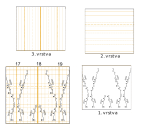
\includegraphics[width=\textwidth]{../img/kap2_drawing_layers}
	\caption{Možné rozdělení obsahu nákresného jízdního řádu na vrstvy}
	\label{fig:spec:njr_vrstvy}
\end{figure}

\begin{figure}[!htb]
	\centering					
	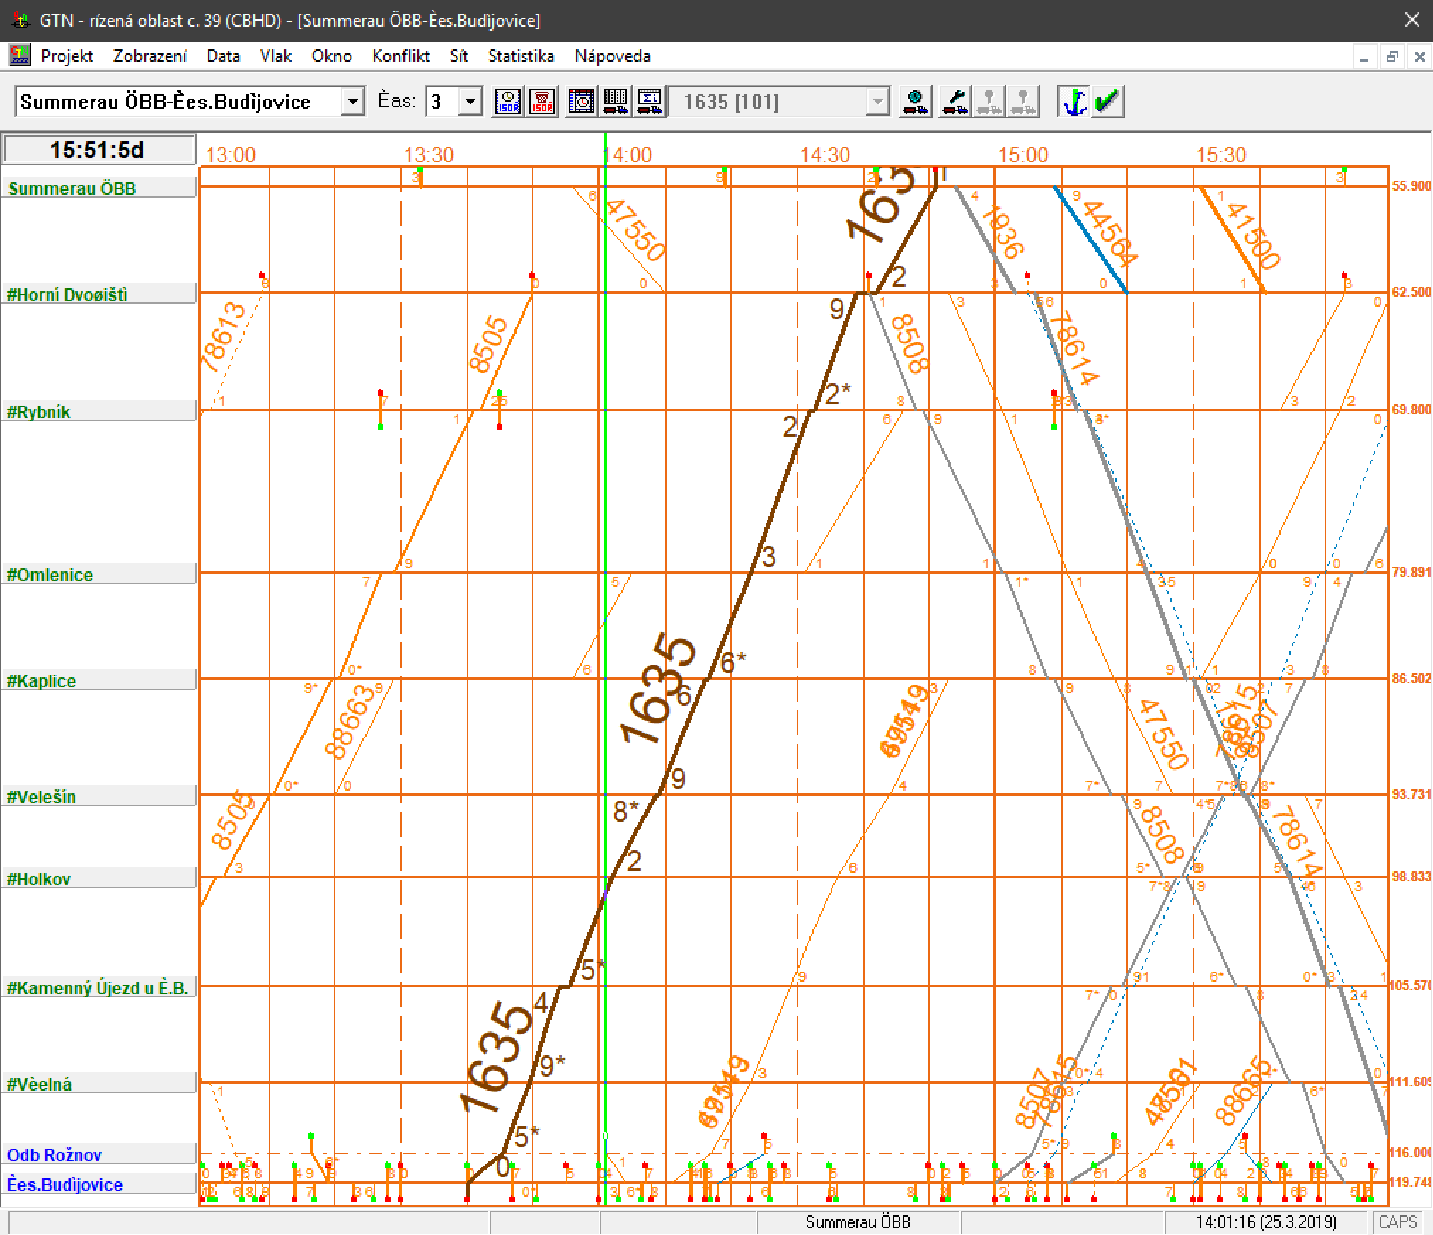
\includegraphics[width=0.7\textwidth]{../img/kap1_gtn_okno_interval_3h}
	\caption{Okno aplikace GTN s~vybraným vlakem vyneseným do popředí}
	\label{fig:spec:gtn_vrstva_vybrany_vlak}
\end{figure}

\newpage
\subsection*{Prvky nákresného jízdního řádu}
\label{kap2:view_elements}
Během změn zobrazení nákresného jízdního řádu je nutné jeho obsah pokaždé znovu vhodně rozmístit. Tento proces nazveme jako \textit{cyklus rozmístění}\footnote{layout cycle}. Pokud například zvětšíme výšku komponenty, zobrazovaný obsah se proporcionálně přerozmístí. Jelikož se změnou výšky změnil i~úhel sklonu šikmých čar, musí se znovu rozmístit prvky jako čísla vlaků nebo informace zobrazované v~ostrých úhlech. 

Některé implementace nákresných jízdních řádů můžou navíc obsahovat složitější konfigurace, které rozmístění komplikují. Dopravní bod například může být místo jedné horizontální čáry reprezentován souborem horizontálních čar, které odpovídají jeho kolejím. Zároveň je možné v~cyklu rozmístění vyhradit úseky kolem dopravních bodů, do kterých se mají umístit informace zobrazené v~ostrých úhlech. Všechny tyto prvky, které reprezentují nějakou část nákresného jízdního řádu a~je nutné je rozmístit, nazveme jako \textit{zobrazitelné prvky}. Základem pro rozmístění všech těchto prvků bude určení jejich velikosti, která může být nastavena různými způsoby, uvedených v~\ref{spec:zobrazitelne_prvky2}.

Pro jednoduchost implementace různých typů nákresných jízdních řádů tak chceme vývojářům umožnit co nejvíce obsahu, který je nutné rozmístit, systematicky popsat pomocí zobrazitelných prvků. S~obsahem nákresného jízdního řádu by pak bylo možné pracovat jako se strukturou stromu, jako na obrázku \ref{fig:prvky_mereni}.

\begin{enumerate}[label=\color{reqcolor}\textbf{R{\arabic*}},resume]
	\item \label{spec:zobrazitelne_prvky1} Obsah nákresného jízdního řádu je možné systematicky popsat strukturou prvků, které označíme jako \textit{zobrazitelné prvky}. Pomocí prvků je možné upravit zobrazení nákresného jízdního řádu v~závislosti na nastavení komponenty.
	\item \label{spec:zobrazitelne_prvky2} Implementace zobrazitelných prvků umožní konfigurovat jejich velikosti různými způsoby:		
\begin{enumerate}
	\item	Prvku může být přiřazena pevná velikost
	\item	Prvku je přiřazena jím požadovaná velikost
	\item	Prvku přiřazená velikost je závislá na nastavení komponenty
\end{enumerate}
 
\end{enumerate}

\begin{figure}[!hbt]
	\includegraphics[width=\textwidth]{../img/kap2_infrastructure_layout}
	\caption{Rozdělení obsahu nákresného jízdního řádu do stromové struktury prvků zobrazení}
	\label{fig:prvky_mereni}
\end{figure}

\subsubsection*{Strategie rozmisťování zobrazitelných prvků}
\label{kap2:strategies_introduction}
Pro některé skupiny zobrazitelných prvků (informace v~ostrých úhlech nebo čísla vlaků) chceme, aby bylo možné vybrat specifické rozmístění, které nazveme \textit{strategií}. Výběr strategie ovlivňuje, kam a~jak moc přehledně se zobrazitelné prvky těchto skupin umístí. Každý typ nákresného jízdního řádu totiž umisťuje tyto zobrazitelné prvky jiným způsobem. Aplikace, s~kterými jsme se seznámili, preferují v~implementaci rozmístění jednoduchost, jelikož většina prostředků a~času strávených jejich vývojem byla určena na implementaci aplikační logiky a~složitější návrh grafické komponenty nebyl při návrhu aplikace zvažován. Knihovna by měla umožnit přehledné rozmisťování zobrazitelných prvků, jelikož se jedná o~vlastnost, která je důležitá pro uživatele aplikací při práci s~nákresným jízdním řádem. S~pomocí obrázku \ref{fig:spec:strategie_cisla_vlaku} si pro ilustraci uvedeme několik přístupů, které se můžou aplikovat při rozmisťování čísel vlaků.

\begin{itemize}
	\item Strategie (a) je nejjednodušší na implementaci. Její jednoduchost spočívá v~tom, že ve většině případů zobrazuje rozmístěné prvky dostatečně přehledně. Náhodně se vybere místo úseku mezi dopravními body, kam se má číslo vlaku umístit. Může ale dojít k~problému, kdy je úsek krátký a~číslo vlaku se bude překrývat s~kótou.
	\item Strategie (b) je dalším jednoduchým způsobem, jak prvky rozmístit přehledně. Strategie se snaží předejít překrývání čísla vlaku s~kótami. Číslo vlaku umístí na střed do nejdelšího dostupného úseku mezi dvěma sousedními dopravními body. Pokud se číslo do úseku nevejde, strategie ho dostatečně zmenší.
	\item Strategie (c) umisťuje číslo na rovnou aproximaci svislé čáry mezi více dopravními body, tak, aby se nepřekrýval s~kótami.
	\item Strategie (d) je použitelná v~případech, pokud vykreslujeme nákresný jízdní řád, který se nemění, jelikož je její implementace náročná na výpočet. Strategie podle složitějšího algoritmu může určit, jak se prvky do nákresného jízdního řádu vhodně rozmístí tak, aby se nepřekrývaly.
\end{itemize}

\begin{figure}[!htb]
	\centering					
	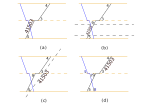
\includegraphics[width=\textwidth]{../img/kap2_strategies_train_numbers}
	\caption{Aplikovatelné strategie při rozmístění čísel vlaků}
	\label{fig:spec:strategie_cisla_vlaku}
\end{figure}

Naše knihovna by neměla mít pevně určené strategie, které se musí používat. Vývojář si tak může zvolit strategii, která mu přijde nejvíce vhodná. Není v~našich silách implementovat všechny možné strategie, ale můžeme knihovnu navrhnout tak, že zásadně ulehčí vytváření dalších strategií. 

Mělo by být možné v~rámci jedné strategie zobrazitelné prvky nahradit jinými, beze změny její implementace. Pro strategii totiž obecně není podstatné, s~jakými prvky pracuje. Všimněme si, že s~prvky pracuje jako s~obdélníky s~pevnou velikostí. Tento proces je zachycen na obrázku \ref{fig:pouziti_strategie}. Strategie nejdříve obdélník změří a~za pomoci operací škálování a~rotace obdélník vhodně umístí. Možnost oddělit strategii od konkrétních zobrazitelných prvků pak umožňuje pro více typů nákresných jízdních řádů použít již existující strategie na jejich specifické zobrazitelné prvky, jako je uvedeno na obrázku \ref{fig:spec:jine_rozmistitelne_prvky}.

\newpage
\begin{enumerate}[label=\color{reqcolor}\textbf{R{\arabic*}},resume]
	\item \label{spec:req:strategie1} Knihovna poskytne nástroje k~implementaci strategií, které rozmisťují zobrazitelné prvky do specifických míst jako ostré úhly nebo oblasti podél svislých čar
	\item \label{spec:req:strategie2} Strategie pracují se zobrazitelnými prvky jako s~obdélníky, jejichž zobrazení a~umístění je možné měnit:
	\begin{enumerate}
		\item Zobrazení prvku je možné strategií upravit transformací rotace
		\item Zobrazení prvku je možné strategií upravit transformací škálování
		\item Prvek je možné umístit na místo určené strategií
	\end{enumerate}
\end{enumerate}

\begin{figure}[!hbt]
	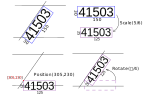
\includegraphics[width=\textwidth]{../img/kap2_strategy_application}
	\caption{Příklad aplikování strategie na zobrazitelný prvek}
	\label{fig:pouziti_strategie}
\end{figure}

\begin{figure}[!htb]
	\centering					
	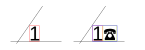
\includegraphics[width=.7\textwidth]{../img/kap2_view_elements_strategies}
	\caption{Možnost použít stejnou strategii na jiné zobrazitelné prvky}
	\label{fig:spec:jine_rozmistitelne_prvky}
\end{figure}

\pagebreak
\subsubsection*{Interakce se zobrazitelnými prvky a~hit-testy}
Jelikož by měla práce s~nákresným jízdním řádem nabízet co největší možnou úroveň interakce, chceme, aby bylo možné při práci s~komponentou pracovat interaktivně i~se zobrazitelnými prvky. Pokud by uživatel aplikace například klikl na kótu nebo prvek zobrazující složitější informace, nějaká jiná komponenta uživatelského rozhraní by na tuto událost mohla zareagovat a~zobrazit dodatečné informace doplňující vizualizaci v~nákresném jízdním řádu. Proces, kdy zjišťujeme, zda se nějaký bod nachází uvnitř rozmístěného geometrického útvaru, se nazývá \textit{hit-testování}.

\begin{enumerate}[label=\color{reqcolor}\textbf{R{\arabic*}},resume]
	\item \label{spec:req:hit-test1} Rozmístěné zobrazitelné prvky je možné otestovat, zda leží na konkrétním bodu plátna
	\item \label{spec:req:hit-test2} Na základě funkcionality \ref{spec:req:hit-test1} bude možné získat všechny zobrazitelné \linebreak prvky nacházející se na specifikovaném bodu plátna podle pořadí vykreslení 
\end{enumerate}

\subsubsection*{Kreslení zobrazitelných prvků}
Jedním ze složitých procesů, který bychom chtěli vývojářům ulehčit, je vykreslování zobrazitelných prvků. Pokud bychom vývojářům, kteří pracují na vykreslování zobrazitelných prvků, poskytli pouze plátno pro celý obsah nákresného jízdního řádu s~nástroji knihovny SkiaSharp, museli by sami do kreslení prvku zahrnout vzniklé transformace a~umístění prvku. Chtěli bychom, aby vývojáři mohli prvky vykreslovat způsobem, kdy by měl každý zobrazitelný prvek přidělené vlastní plátno na kreslení a~vykreslení by tak probíhalo nezávisle na zobrazení v~nákresném jízdním řádu.

\begin{enumerate}[label=\color{reqcolor}\textbf{R{\arabic*}},resume]
	\item \label{spec:zobrazitelne_prvky_vykresleni} Pro vykreslení obsahu zobrazitelného prvku je vytvořeno plátno, které odpovídá velikosti prvku. Vykreslení prvku tak probíhá nezávisle na celém zobrazení nákresného jízdního řádu.
\end{enumerate}

\subsection*{Základní model obsahu nákresných jízdních řádů}
\label{kap2:req:model_impl}
Jelikož nákresné jízdní řády mají mnoho společných vlastností, v~rámci splnění cíle \ref{uvod:cil:knihovna} \ref{uvod:cil:knihovna:ruzne_typy_njr} bychom chtěli vytvořit implementaci základního modelu nákresných jízdních řádů. Jejím rozšířením bude možné vytvořit konkrétní typ nákresného jízdního řádu. V~rámci základní implementace poskytneme vývojářům implementaci několika strategií.